%% INIZIO CONTENUTO TESI
%% TODO: Create a section where to explain the system's teminology.
%% * Any term inside the section will be start with the capital letter
%% * (es. Archived, Annotation, etc.)
\mainmatter
\chapter{Introduzione}
\label{cap:introduzione}

\section{L'azienda}
Lo stage formativo si è tenuto presso l'azienda Wonderflow, fondata nel 2014
ad Amsterdam. Wonderflow si colloca nel mercato \gls{B2B}
offrendo alle aziende una \gls{dashboard}, denominata \textbf{Wonderboard}, in
cui le compagnie registrano i loro prodotti e ottengono una serie di
statistiche sull'andamento del gradimento e commenti degli utenti utili per
poter migliorare i propri articoli.

\begin{figure}[htbp]
\begin{center}

\includegraphics[height=2cm]{wonderflow-logo}
\caption{Logo Wonderflow}
\end{center}
\end{figure}

\subsection{I ruoli}
La Wonderflow è suddivisa in tre gruppi: analisti, sviluppatori e venditori.

E' importante comprendere il ruolo dell'\textbf{analista} e dello
\textbf{sviluppatore}, all'interno dell'azienda ed il loro modo di lavorare, in
quanto l'intera esperienza di stage gira attorno a queste due figure.

\subsubsection{Analisti}
La raccolta delle informazioni sui prodotti è compiuta dal team di
\textbf{analisti} attraverso l'analisi delle recensioni di un prodotto, prese
da vari siti web di vendita, al fine di individuare frasi chiavi in cui
emerge un \textbf{sentimento}, denominate \textbf{annotazioni}.

L'analisi delle recensioni avviene attraverso un \textbf{editor} interno dove
l'\textbf{analista} è in grado di sottolineare, attraverso la selezione del 
testo con il mouse, l'annotazione presente nella recensione. Una volta 
individuata l'annotazione e associato un sentimento, potrà essere salvata 
nell'archivio online della Wonderflow.

Vi sono altri aspetti nella creazione delle annotazioni ma verranno trattati
nel capitolo dedicato all'esposizione del progetto in modo da avere un contesto
adeguato. Per quanto riguarda la procedura d'elaborazione delle annotazioni per
ottenere i dati visualizzati dalla Wonderboard, questa non verrà trattata in 
quanto fuori dall'argomento dello stage.

\subsubsection{Sviluppatori}
Il gruppo \textbf{sviluppatori} realizza gli strumenti software usati
internamente all'azienda e scarica le recensioni per poi fornirle agli analisti.

Data il loro ridotto numero, le conoscenze si espandevano per una buona parte
 dell'organizzazione, in modo da andare incontro alle esigenze dell'azienda.
Non era inusuale che ad un programmatore venisse richiesto di conoscere il 
flusso di lavoro dell'analista o apprendesse tecniche di vendita o prendesse 
decisioni sull'impostazione dell'azienda. Tutto ciò aumentava il senso di 
appartenenza ed importanza della persona dentro il contesto aziendale, oltre
che dare la possibilità di comprendere meglio i bisogni interni.

Le interazioni tra sviluppatore e analista, o venditore, avvengono in modo
diretto, non formale e senza passare per un ente supervisore. In questa maniera
la comprensione dei requisiti diventava più veloce; si generava un rapporto tra
i membri dell'azienda più stretto ed un ambiente di lavoro più rilassato.

L'organizzazione dei compiti assegnati sono auto-organizzate dall'assegnatario.
Lo sviluppatore decide come affrontare un problema, progettare la soluzione ed
implementarla usando le risorse a disposizione. Il motivo è lasciare libertà ai 
nuovi sviluppatori in modo da portare dentro alla compagnia il proprio bagaglio 
di conoscenze. L'approccio libero è principalmente pensato per personale 
giovane con più alta probabilità di condividere e applicate idee e metodologie 
al passo coi tempi.

\section{L'organizzazione}
Da come si può dedurre dalla descrizione sopra la Wonderflow, come tante altre
case produttrici di software, aderisce al metodo di sviluppo \gls{agile} ed 
utilizza \gls{scrum}, figura \ref{fig:scrum_process}, come modello di ciclo di 
sviluppo.

\begin{figure}[ht]
\begin{center}
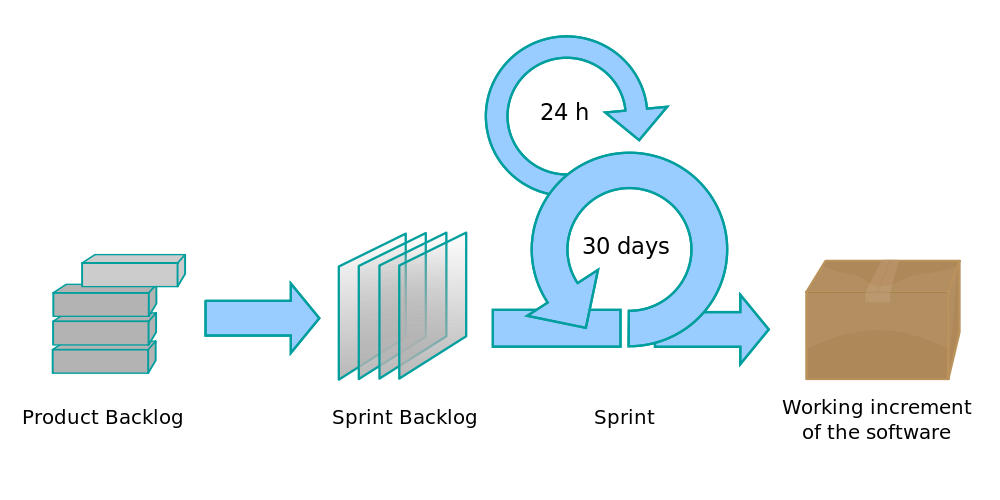
\includegraphics[height=5cm]{scrum_process}
\caption{Rappresentazione modello di sviluppo Scrum}
\label{fig:scrum_process}
\end{center}
\end{figure}

\subsection{Attività giornaliere}
Seguendo \gls{scrum}, ogni giornata lavorativa inizia con lo
\textit{standup meeting}. Attraverso il programma di messaggistica 
\textit{Slack} si invia il riassunto delle attività svolte il giorno prima,
quelle che si andranno a compiere il giorno stesso ed eventuali ostacoli che
presumibilmente si incontreranno. Una volta terminato il \textit{meeting} si 
inizia con lo sviluppo fino all'ora fissata per il \textit{daily}, una riunione 
generale dove \textbf{ogni} membro della compagnia è chiamato a presentare agli 
altri il lavoro svolto durante la giornata, lo stato attuale dei compiti, 
difficoltà trovate e i dubbi sorti.

\subsection{Sviluppo}
L'unita di tempo in cui si effettua il lavoro si chiama \gls{sprint}.
Nello scenario dello stage, il \textit{tutor} aziendale ha dimensionato 
lo \gls{sprint} della durata di una settimana in cui svolgere un aspetto del
progetto ed integrarlo nel sistema aziendale una volta concluso.
La chiusura dello \gls{sprint} implica una prima fase di \gls{verifica} per 
accertare che il codice prodotto sia conforme agli standard dell'azienda. 
Nel caso d'esito positivo il prodotto finale viene rilasciato, altrimenti viene
trascritta la lista dei difetti riscontrati e da risolvere, ritornando cosi allo
sviluppo. Una volta apportate le modifiche correttive verrà ricondotta la 
verifica. Questa procedura continuava finché il risulto non fosse confacente 
alle aspettative.

Le norme fissate dalla Wonderflow mirano nell'avere il codice il più
comprensibile possibile in modo che futuri sviluppatori siano capaci, in poco
tempo, a lavorare con esso ed in completa autonomia. Le caratteristiche che si
vanno ad ispezionare sono:
\paragraph{Logica}
E' importante non produrre algoritmi complessi che potrebbero richiedere un
certo quantitativo di tempo per studiarli e comprenderli. Meglio produrre
programmi semplici adattati ``ad hoc'' per la situazione.

\paragraph{Nomi}
I nomi per le variabili, funzioni, classi, ecc... devono essere comprensibili
e fornire al lettore un'idea del suo scopo. Inoltre i nomi delle funzioni
devono dare una qualche informazione sui suoi parametri per colmare l'assenza
di documentazione. Il motivo di queste scelte è l'utilizzo del linguaggio 
JavaScript, non tipato e con nessun immediato riferimento alle proprietà degli
attributi vincolato dalle regole sintattiche.

\paragraph{Organizzazione}
Dividere il progetto in vari file (uno per classe) e raccoglierli in cartelle
denominate in base all'area tematica toccata. La norma mira ad aiutare ad 
orientarsi durante lo sviluppo.

\paragraph{Progettazione}
Per garantire un semplice utilizzo dei vari progetti realizzati è importante
soddisfare due fattori: \textbf{dimensione} e \textbf{semplicismo}.
La prima è tanto più buona quanto è più ridotta. Progetti di piccoli dimensioni
sono facili da gestire, comprendere e risultano maggiormente mantenibili. E'
inoltre possibile poter agilmente cambiare lo sviluppatore che ne fa uso
garantendo l'indipendenza sul personale.

Per quanto riguarda la seconda, vengono apprezzate maggiormente soluzioni di
\textit{design} non elaborate e di facile comprensione, sempre per acconsentire
una rapida comprensione del software.

Il principale obiettivo é produrre codice comprensibile. Spesso la
soddisfazione dei requisiti appena descritti non corrisponde ad un risultato
completo e caratteristiche come la resilienza, robustezza o estendibilità
potrebbero essere assenti, almeno nelle prive versioni. Il tempo dedicato
alla progettazione iniziale veniva ridotto in favore di rilasci più frequenti,
con l'uso continuo del \gls{refactoring}.

E' importante sottolineare questi aspetti in quanto si riflettevano
inevitabilmente sulle varie scelte compiute nello svolgere le varie mansioni
dello stage.
